\chapter{Introduction}
\label{chp:chp1}

Our brain is our most precious, yet most mysterious organ. It consists
of 100 bilion neurons, each neuron typically having 10 000 connections
of lengths of up to a meter. As such, it is a intricate web in which
and with which we experience the world. In addition to the neurons,
the brain consists of about the same number of glial cells, around 700
km of blood vessels, and the extracellular matrix, and it is
surrounded by the clear water-like cerebrospinal fluid, which
alltogether work to maintain the delicate neurons' environment in a
healthy state. Given the vast numbers of neurons, glial cells and
blood vessels, a natural approach to understand the brain's physiology
and function is through continuum-based modelling.

%% \mer{I think we need to refine this (but keeping it here for later).}
While there are many applications of continuum-based brain modelling, our
motivation in writing this book and the corresponding software tools  comes from recent theories 
concerning the restorative mechanisms of sleep. Here, recent theories 
consider the brain as a poro-elastic medium, where the elastic medium consists of the cells
and the fluid is the extra-cellular matrix (of course also hyper- and visco-elastic 
materials~\cite{goriely2015mechanics, budday2019fifty} could be considered). 
In this setting, a paradigme shift was introduced by the glymphatic theory, proposed and developed over the last 8 years by the 
groups of Iliff and Nedergaard, which proposes that
extra-cellular diffusion, as described in the seminal work
of Sykov{\'a} and Nicholson~\cite{sykova2008diffusion}, is
not sufficient to explain the fundamental processes of metabolism of the brain. 
In particular, pressure driven convective flow  is
required to wash away the larger molecules of the metabolic waste products
produced during the day~\cite{iliff2012paravascular,
  jessen2015glymphatic, xie2013sleep}. Importantly,  if the metabolic waste 
if not removed it accumulate as seen  in patients with  Alzheimer's disease. 
As such this topic has received a lot of attention from the modeling 
community concerning the mechanisms at the micro-scopic level,
c.f. e.g., ~\cite{aldea2019cerebrovascular, daversin2020mechanisms, diem2017arterial, 
holter2017interstitial, ray2019analysis, sharp2019dispersion, smith2017test}, to name a few. 
However, very few works address the macroscopic level and how to employ modelling in a patient-specific
manner, see e.g., ~\cite{chou2016fully, lee2019mixed}. Crucial to achieve patient-specific assessment 
is mesh generation based on medical images and typically integration of several different images
of different types. Our intention with this book is to equipp the reader with 
software tools to perform such studies.   

Obviously, there are many other applications involving continuum based models of the brain's physiology. 
For instance, alternative macroscopic theories which involve prion related development of Alzheimer's 
disease has been proposed~\cite{fornari2019prion, kevrekidis2020anisotropic}. 
Another interesting observation is the fact that    
astronauts often experience
visual impairments and are at risk of developing early dementia as a
consequence of their periods in low or zero gravity. The reason seems
to be intracranial pressure changes and a shift in fluid volumes in
intracranial compartments~\cite{alperin2018spaceflight}. 
Another well-known computational modeling problem is  motivated by epilepsy.  Here, 
the inverse EEG problem of determining the source of the epileptic seizure 
as an inverse problem involving an elliptic PDE~\cite{grech2008review} is a hot research topic. 
Many other applications and developements could of course be mentioned. 

% \KAM{Should include epilepsy, Alain's prions and stroke as well.}

This book will not dive to any dept into any of the applications mentioned above,  but we
wish to enable personalized continuum-based modeling in an accessible
manner. You, the reader of this book, will learn how to formulate,
set-up and implement mathematical and computational models of brain
biophysics in patient-specific geometries using finite element
simulations and MR images (see Figure \ref{fig:chp1:pipeline}). We
will use the evolution and distribution of a solute concentration due
to diffusion as a model problem, and increase the complexity of the
data and techniques involved in the course of the book. Of course,
the process involves several challenges and pitfalls which will be
outlined.

\begin{figure}[t]
  \begin{center}
  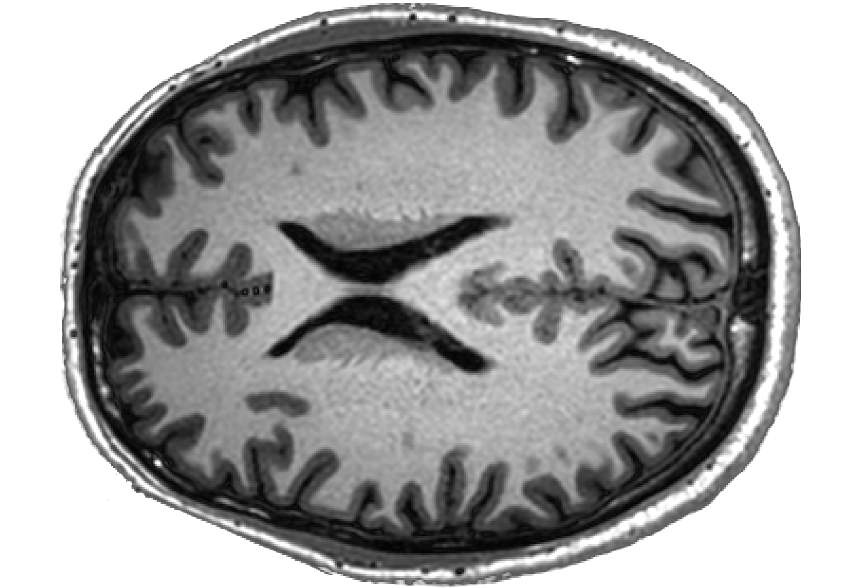
\includegraphics[height=2.3cm]{./chapters/chp1/FIG/T1-image-rot-white}
  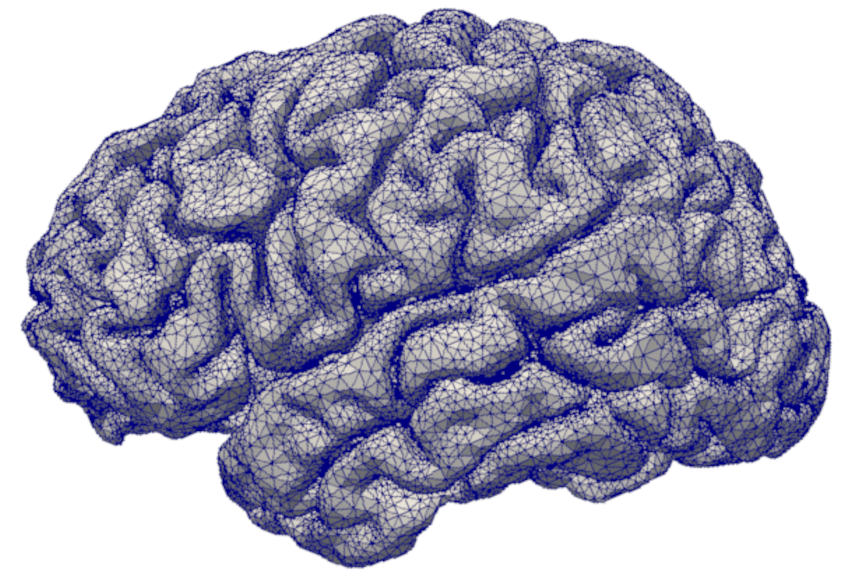
\includegraphics[height=2.3cm]{./chapters/chp1/FIG/ernie-volume-64}
  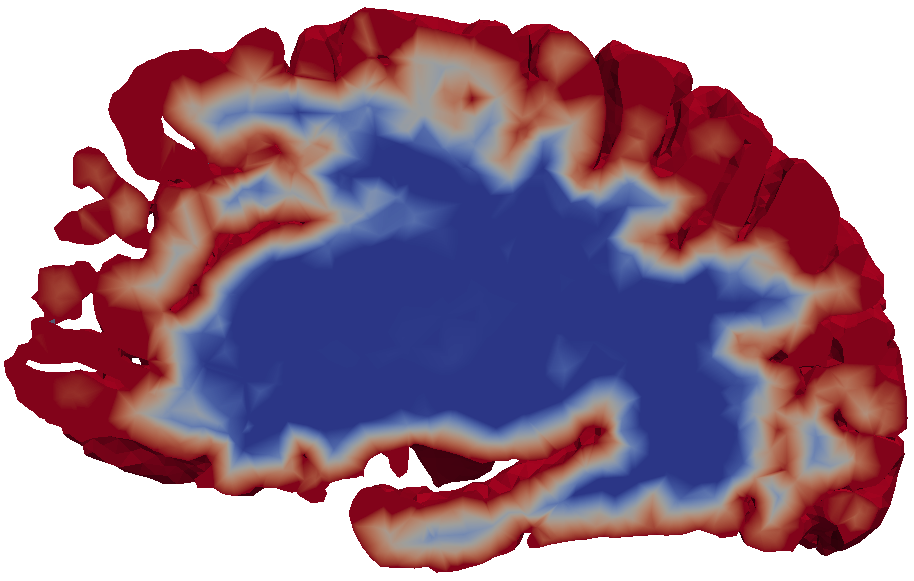
\includegraphics[height=2.3cm]{./chapters/chp1/FIG/soltn-t30-crop}
  \hfill
  \end{center}
  \caption{Going from magnetic resonance images (MRI) of a human brain
    to a numerical simulation of a biophysical phenomenon. From left
    to right: (a) a MR image of a human brain viewed along the axial
    direction, (b) a finite element mesh extracted from the T1 image,
    (c) a snapshot of a tracer distribution simulation over this mesh.}
  \label{fig:chp1:pipeline}
\end{figure}

\section{A model problem}

Suppose that we aim to study the diffusion of a solute concentration
in a region of the brain. The region $\Omega$ could represent the left
brain hemisphere or a smaller region such as the hippocampus, while
the concentration $u$ could represent an injected tracer used in
imaging (such as gadubutrol~\cite{ringstad2018brain} or
dextran~\cite{iliff2013cerebral}) or possibly a metabolic waste
protein associated with neurodegenerative disease such as
amyloid-$\beta$ or tau. We can describe this model problem by a
time-dependent partial differential equation (PDE): find the
concentration $u = u(t, x)$ at spatial points $x \in \Omega$ and time
points $t > 0$ such that
\begin{subequations}
  \label{eq:diffusion}
  \begin{align}
    \label{eq:diffusion:a}
    u_t - \Div K \Grad u &= f &&\text{ in } (0, T] \times \Omega, \\
    \label{eq:diffusion:b}
    u &= u_d && \text{ on } (0, T] \times \partial \Omega, \\
    \label{eq:diffusion:c}
    u(0, \cdot) &= u_0 && \text{ in } \Omega.
  \end{align}
\end{subequations}
In the diffusion equation~\eqref{eq:diffusion:a}, $u$ is the unknown
field, while $K$ is the diffusion tensor coefficient and $f$
represents any source or sink for the concentration within the
domain. The subscript $t$ denotes the time derivative, $\Div$
represents the divergence and $\Grad$ the spatial gradient. The second
equation~\eqref{eq:diffusion:b} gives a boundary condition: the
function $u_d$ represents a known distribution of the concentration on
the boundary $\partial \Omega$ for all times. The third
equation~\eqref{eq:diffusion:c} gives an initial condition for the
solute concentration: the function $u_0$ represents the known initial
concentration distribution throughout $\Omega$ at $t=0$. The combined
problem \eqref{eq:diffusion} is a complete initial boundary-value
problem and will be our model problem.

%% The remainder of this text describes the use of  
%% T1-weighted MRI images (Figure~\ref{fig:chp1:mri} (left)) to create a 
%% computationally-friendly representation of the brain.   
%% T2-weighted MRI images (Figure~\ref{fig:chp1:mri} (center)) can be used 
%% to augment the mesh generation process and enhance that computationally-friendly
%% representation, as needed.  Finally, diffusion-weighted MRI images 
%% (Figure~\ref{fig:chp1:mri} (right)) will be used to construct our diffusion tensor, 
%% $K$, and the open-source FEniCS numerical software package  is employed to 
%% solve \eqref{eq:diffusion} using the data-derived components.


%In this chapter the primary goal is to demonstrate the simplest case of
%computational human brain modeling. We will use basic features of  
%the tools overviewed in Chapter \ref{sec:chp2:tools} to create a 
%simple left-hemisphere human brain mesh from MRI data. We will use this mesh
%to solve a simple problem; namely to find $u = u(t,x)$ so that 
%\begin{align}
%  \label{eqn:chp3:model-problem}
%	&\partial_t u -\Div\left(\tnsr{K} \Grad u\right) = f,\\
%	u=u_d(t,x) &\text{ on } (0,T]\times\partial\Omega, \quad u(0,x) = %
%	u_0(x)\text{ on }\Omega.\nonumber
%\end{align}

%The problem \eqref{eqn:chp3:model-problem} is a basic initial value problem 
%motivated by clinical application.  Namely it is a basic starting point, for 
%example, when considering models for tracking the diffusion of a substance, such 
%as a tracer or amyloid-$\beta$ protein concentration, through the brain.  The 
%function $u_d(t,x)$ represents the value of the substance concentration on the 
%boundary, $x\in \partial\Omega$, for times $0<t<T$ where $T$ is a fixed 
%end-point, in time, of interest; for example, the end time of the tracer 
%experiment. The function $u_0(x)$ represents the initial tracer distribution 
%in the entire left hemisphere and $f=f(t,x)$ represents a source term for 
%additional tracer concentration injection.  In the present chapter, $\Omega$ 
%will represent the left hemisphere of the brain and $\partial\Omega$ is 
%the corresponding boundary.
%
%In this particular chapter we will assume that $K$ is a constant value 
%which, in practice, it certainly is not.  However, our purpose here is to 
%produce a simple computational code to serve as a foundation for 
%further increasing complexity using patient MRI data. 
%
%The purpose of this chapter is to offer a  high level overview
%regarding the basic data files and tools needed throughout the remainder of the 
%text.  Further chapters delve into specifics related to these files and 
%tools, as necessary, to accomplish specific goals.  In order to facilitate a 
%broad discussion it is helpful to have in mind a concrete, albeit simple, 
%mathematical modeling problem.  Suppose we would like to study the distribution
%of a certain solute concentration throughout a domain, $\Omega$, consisting
%of brain tissue matter.  This concentration could represent, for example,  an 
%injected tracer or possibly a waste protein, such as amyloid-$\beta$ or 
%phosphorylated tau, that we are interested in tracking.  A very simple 
%starting point for a mathematical model could then look similar to 
%the following:
%
%\begin{equation}
%  \label{eq:chp1:poisson}
%  -\Div\left(\tnsr{K} \Grad u\right) = f \quad \mbox{in} \ \Omega.
%\end{equation} 

%------------------------
%\mer{@TT: Is the next paragraph necessary? I find it a bit repetitive and
%  sometimes inaccurate (we do not likely know the source/sink function $f$
%  do we?) I suggest we drop it.}
%  
% Action: removed
%The unknown quantity, for which we hope to gain information by solving
%\eqref{eqn:chp1:model-problem}, is $u$.  However, there are 
%other physical quantities, namely $\tnsr{K}$ and $f$, involved in such a simple 
%expression. If we are modeling an experiment then we are likely to know the 
%nature of the source function, $f$, as this is quantity we may either control or 
%possess the necessary outside information regarding it.  The quantity $K$ is called 
%the diffusion tensor and dictates the flow pattern of extracellular fluid in the 
%brain; this quantity is complex and heavily dependent on the of axonal bundles 
%in the brain. Moreover, the domain $\Omega$ is not a mathematical abstraction; 
%we want $\Omega$ to coincide with some area of the brain; the geometry of the 
%domain needs to match the physical reality of the tissue structure inside the 
%skull of the patient in question.  We certainly have no real a priori knowledge 
%of these two aspects of \eqref{eqn:chp1:model-problem} for any particular patient.
%-----------------------------

%-----------------------------
%\mer{@TT: Next paragraphs are good addition. Something along these lines
%  is nice. But perhaps we can condense it a bit? I try to avoid
%  formulations of the form "something called X" e.g. "a mathematical
%  technique called the finite element method". I think we can be bold
%  and precise right away instead :-)}
%
% Action: condensed.

%In practice, what we do have is clinical images such as the magnetic resonance 
%images shown in Figure \ref{fig:chp1:mri}.  Thus, too solve 
%\eqref{eqn:chp1:model-problem}, and ultimately obtain a meaningful 
%result for the function $u(t,x)$, we need to somehow extract knowledge of 
%$K$ and $\Omega$ from these types of clinical image data.  How can we go about 
%this process?  This is the central question that this book will address.  Once 
%we have this information we would also like to know how to set up and solve 
%\eqref{eqn:chp1:model-problem} using pre-existing software; this is our secondary 
%objective.  It would be preferable to avoid unnecessary, and quite non-trivial, 
%algorithm implementation; so we prefer to use software that has already been 
%developed by experts in this area.  
%-------------------------------

%for $u(x,t)$; c.f.~Figure \ref{fig:chp1:mri} (right).  % 
%%Thus, to solve 
%%\eqref{eq:diffusion}, for $u(x,t)$, we must extract $K$ and $\Omega$ 
%%from the imaging data. 
%How can we do this this? This is the central question that we 
%address.  Our secondary objective is to demonstrate the use of pre-existing 
%software in order to setup and solve \eqref{eq:diffusion}.
%
%Once we have the information, we want to set up and solve 
%\eqref{eq:diffusion} using pre-existing software; this is our secondary 
%objective.    
%
%
%
%\mer{@All: How about we have (a) MR image, (b) Plot of mesh, and (c)
%  Plot of solution here?}
%
%

%connect these quantities to the `real-world' of 
%medical data; furthermore, how can we extract such information from the 
%data-sets typically produced by medical procedures?  
%
%Medical data, such as those provided by magnetic resonance imaging (MRI),
%play an enormous practical role in the ability of applied mathematicians to 
%extract the necessary information enabling models such as 
%\eqref{eq:chp1:poisson}.  Take, for example, 
%$\tnsr{K}$ in \eqref{eq:chp1:poisson}.   Mathematically, 
%this quantity is a matrix that, at each point $x\in \Omega$, offers information 
%on the tendency of $u$ to flow; that is, in what direction $u$ is more or less 
%free to travel.  We will see that information about $\tnsr{K}$ can be extracted 
%from so-called diffusion tensor image (DTI) data.  Likewise, $f$ 
%in \eqref{eq:chp1:poisson} mathematically represents a 
%so-called source or sink of $u$; depending on the context this could be an injected
%dye tracer or possibly proteins carried into the parenchymal interstitium 
%via paravascular spaces.  
%We will see that information about $f$ can be 
%ascertained from so-called arterial spin labeled (ASL) image data.

%A more fundamental problem, however, is one of constructing a computational
%representation of the brain, i.e. $\Omega$ in \eqref{eq:chp1:poisson},  on which we can solve 
%\eqref{eq:chp1:poisson} to begin with; $\tnsr{K}$ and
%$f$ notwithstanding.  A computational representation of the physical brain 
%is referred to as a mesh.  An MRI machine utilizes time varying electromagnetic fields to 
%create images which discriminate   
%between different areas of the brain in terms of different structure or function.  
%We will see that images obtained by a standard protocol called T1-weighted MRI
%can be used to extract the data necessary to create a preliminary 
%computational-mesh-representation of the brain.  We will also see that 
%another standard protocol called T2-weighted MRI  can be used to augment this mesh generation
%process and enhance the resulting computational mesh when needed. 


%Introductory discussion on the datafiles in the context of the model problem 
%\begin{equation*}
%	-\Div(K\Grad u) = f
%\end{equation*}
%what data files will give us which pieces of the infrastructure to solve 
%the above?  How will we use the basic tools in order to get the requisite
%pieces?
%
%\begin{itemize}
%	\item High level explanation of the MRI procedure
%	\item High level explanation of the end goal (producing a mesh %
%		on which a PDE can be solved)
%	\item{ High level explain T1 and T2 images
%		\begin{itemize}
%			\item What do the do for us / connection to PDE
%			\item Give a few examples
%			\item Explain the deficiences (low resolution ventricles)
%			\item Explain how T2 images can help overcome the above
%		\end{itemize}
%	}
%	\item{ High level explain DTI images
%		\begin{itemize}
%			\item What do they do for us and connection to PDE
%			\item an example
%			\item Explain any shortcomings / what they don't do well
%		\end{itemize}
%	}
% \end{itemize}
%


% -------- DONE ----------
%\begin{itemize}
%\item
%  Introduce equation and MRI images side-by-side and explain that we
%  want to link these.
%\item
%  Outline of the chapters?
%\end{itemize}

\section{On reading this book}

This text assumes basic knowledge of partial differential
equations. For instance, the diffusion equation \eqref{eq:diffusion}
is a classical continuum-based partial differential equation with
well-known behaviour in both the mathematical and numerical sense. A
reader unfamiliar with this equation is advised to first consult an
introductory text on solving partial differential equations using the
finite element method~\cite{tveito2004introduction,
  langtangen2016solving, gockenbach2006understanding,
  langtangen2019introduction}.

It is assumed that the reader is comfortable executing commands from a
command line in a terminal window (which is also canonically referred
to as called a command window or command prompt). Terminal commands
will throughout be formatted as:
\terminal{\$ cd ..}
\noindent Operating-system (OS) level commands, such as the one above, may
differ from OS to OS and that the user will need to resolve the
specific instruction necessary to complete OS-level directives with
respect to their choice of platform.

We also assume that reader is familiar with the fundamentals of the
Python programming language or, alternatively, can understand the
syntax well enough to follow the source code that appears throughout;
we will not use any advanced Python programming techniques. We use
Python 3 throughout, and thus we must ensure that we have Python
version 3.0 (or preferably any later version) installed. You can check
your Python version by either of the terminal commands:
\terminal{\$ python {\ddash}version \\
\$ python3 {\ddash}version
}
We will make use of Python interface to the FEniCS Project finite
element software~\cite{alnaes2015fenics}, and we assume that the
reader is familiar with the material covered by the FEniCS
tutorial~\cite{langtangen2016solving}.

%-----------------------
%\mer{@TT: Do we need this section? I think this is material that we should assume that the reader is familiar with, and we can refer to an introductory text to PDEs instead. }
% Action: removed
%-----------------------
%\subsection{Basic Notation}
%We assume that the reader is, more or less, familiar with the basic mathematical 
%notation of Calculus.  We will use some consistent mathematical 
%throughout the text that we now briefly recount.  The symbol $\Omega \subset \R^3$ 
%will be used to signify a domain of interest; relevant to the context of whatever 
%discussion is at hand.  This could be the whole brain, a single hemisphere, 
%a small region such as the hippocampus, or the ventricles, etc. The notation 
%$\partial\Omega$ will always represent the two-dimensional surface boundary 
%of the domain $\Omega$. Partial derivatives 
%with respect to a variable, such as time $t$ or a spatial direction $x$ or $y$, 
%will be represented as $\partial_t$, $\partial_x$, $\partial_y$, etc.  
%We will use $\Div$ to represent the divergence of a vector $v = (v_1,v_2,v_3)$ as
%\[
%\Div v = \partial_x v_1 + \partial_y v_2 + \partial_z v_3,
%\]
%and the symbol $\Grad$ will denote the usual gradient of a scalar quantity as 
%\[
%\Grad f = (\partial_x f, \partial_y f, \partial_z f).
%\]
%We will refer to time as a real variable over an interval in $\R$.  The use of 
%$T$ will always indicate some arbitrary, but fixed, end time.  Thus, we may 
%encounter statements akin to $t\in(0,T]$, to indicate that zero is not included, or $[0,T]$ to indicate 
%the inclusion of $t=0$ in the time domain.  Beyond this, no further symbolic familiarity 
%is needed with the exception of the usual integral notation from elementary 
%Calculus. 

\section{Data sets and scripts}

The data sets and scripts used and described in this book are openly
available on Zenodo:
\begin{itemize}
\item
  The book data set, including MR images, can be downloaded from \\
  \url{http://doi.org/10.5281/zenodo.4386987}~\cite{kent_andre_mardal_2020_4386987}.
\item
  The book scripts can be downloaded from \\
  \url{http://doi.org/10.5281/zenodo.4386998}~\cite{kent_andre_mardal_2020_4386999}.
\end{itemize}
 We strongly recommend that you download and unpack these materials before
 reading further.

%\subsection{External dependencies}
\index{Ubuntu}
We will use a number of external tools in this book. Most of these
tools are available for a number of operating systems, with separate
installation instructions and dependencies for each system. For the
key external tools, we here provide installation instructions on Linux
Ubuntu (version 20.04, but earlier or later versions might also work
fine). Whenever we refer to an Ubuntu specific terminal command, we
format this as:
\ubuntu{\$ sudo apt-get install ... }
\noindent We note that before installing packages it can be important to update
the Ubuntu package list. This can be done by the following (Ubuntu-specific)
terminal command:
\ubuntu{\$ sudo apt-get update}
\noindent For other operating systems, we refer to the specific
software documentation for installation instructions.

%% \section{An outline of the remaining contents of the text}
%% This book presents the steps needed to develop and solve continuum based, patient-spesific
%% models in a more-or-less step-wise fashion.  
%% Each chapter demonstrates one major component of extracting, from clinical data, the 
%% relevant quantities needed to solve for instance \eqref{eq:diffusion}. The overall flow 
%% of the book is to first, either introduce a method for extracting data from a 
%% clinical image or to improve on an entity already extracted from data; second, we 
%% will periodically stop and turn our attention to solving a problem 
%% similar to \eqref{eq:diffusion} using what we have learned thus far.




%% \COMMENT{
%% \section{Moved from Chap 3}

 
%% After each piece of data is extracted we will demonstrated how that data can be 
%% used by solving a simplified version of \eqref{eqn:chp1:model-problem} that requires 
%% no further considerations. We will slowly add complexity to our model problem as 
%% we progress.   

%% Now that we have constructed our mesh of the left pial surface this section
%% details the solution of the model problem \eqref{eqn:chp3:model-problem}.  Our
%% first model is quite simple; both practically and mathematically.  From a 
%% practical point of view we are at this point using a mesh that 
%% does not resolve different brain substructures; such as the gray and 
%% white matter.  From a mathematical point of view, problem 
%% \eqref{eqn:chp3:model-problem} is one of the most well studied problems in 
%% science and mathematics.  Despite the simplicity of \eqref{eqn:chp3:model-problem} %
%% it is still related to questions of clinical interest.  For example, the so-called %
%% `amyloid-$\beta$ hypothesis' \cite{selkoe-2016-journal} suggests a connection %
%% between the progression of Alzheimer's disease and the collection of the toxic %
%% protein amyloid-$\beta$, also phosphorylated tau, in different brain regions.  

%% To track the movement of such proteins in the brain researchers have used equations 
%% similar, in presentation, to \eqref{eqn:chp3:model-problem}.  One example is 
%% the recent use of the Fisher-Kolmogorov-Petrovsky-Piskunov, 
%% or Fisher-KPP, equation \cite{goriely-2018-journal} coupled to a morphoelastic
%% model of the brain deformation to simulate the affect of protein diffusion
%% and atrophy in Alzheimer's progression; the Fisher-KPP model is given by 
%% \begin{equation*}
%% \partial_t u - \nabla\cdot\left(K\Grad u\right) - \alpha u(1-u) = 0,
%% \end{equation*}
%% where $K$ is, in general, a transversely anisotropic diffusion tensor and 
%% $\alpha > 0$ is a growth rate.  Now, equation \eqref{eqn:chp3:model-problem} 
%% does not satisfy the $\alpha > 0$ requirement; even in the case of $K$ constant
%% and isotropic.  However, the point here is that \eqref{eqn:chp3:model-problem}
%% is a reasonable `first starting point' based on the current state of the art 
%% approaches employed in contemporary modeling practice. % 
%% %
%% %In fact, an equation 
%% %somewhat resembling \eqref{eqn:chp3:model-problem}, the Kolmogorov-Petrovsky-Piskunov 
%% %equation, has recently \cite{goriely-2018-journal} been coupled to a sophisticated 
%% %eslastic model of the brain in order to simulate the impact of the location of 
%% %first appearance of toxic proteins on the long-time development of diseases 
%% %such as Alzheimer's disease.
%% %
%% Another interesting question, of current clinical debate, is that of how 
%% waste proteins generated in the brain, such as amyloid-$\beta$, make their way
%% out into the cerebrospinal fluid (CSF) where they may be cleared; either by 
%% traditional lymphatic vessels or other mechanisms.  In fact the recent %
%% `glymphatic hypothesis' \cite{bacyinski-2017-journal,iliff-2012-journal} suggests %
%% a method of CSF circulation in the brain that may act as a kind of % 
%% `interior lymphatic system'; cleaning waste molecules, such as amyloid-$\beta$, 
%% out of the brain parenchyma.  

%% \kent{I don't think we should include the non-linear term. 
%% Should perhaps say something about bc.}

%% \mer{Think about moving a bit later.}

%% A recent clinical experiment \cite{ringstand-2018-journal} has aimed to test the communication
%% of the subarachnoid CSF compartment and the extravascular component of human 
%% brain tissue; such communication is postulated by the glymphatic hypothesis.  The 
%% study was conducted using MRI imaging alongside the injection of a tracer into
%% the subarachnoid CSF.  Following injection, the clinicians then observe how the 
%% tracer makes its way through the brain and examine the time-to-clearance of this
%% tracer for both reference patients and a cohort with dementia.  
%% }
